% !TeX root = ../main.tex
\chapter{Detailed Sequence Diagrams}
\label{appendix:sequence-diagrams}

This appendix collects detailed sequence diagrams and auxiliary
operational flows for the main asynchronous and cross-runtime behavior
of the system. The LTI Launch sequence is kept in
Chapter~\ref{chap:phan-tich-thiet-ke} because it is central to the
security and integration argument; all other sequences live here.

\section{Document Upload and Processing}
\label{appendix:seq-document}

\begin{figure}[H]
    \centering
    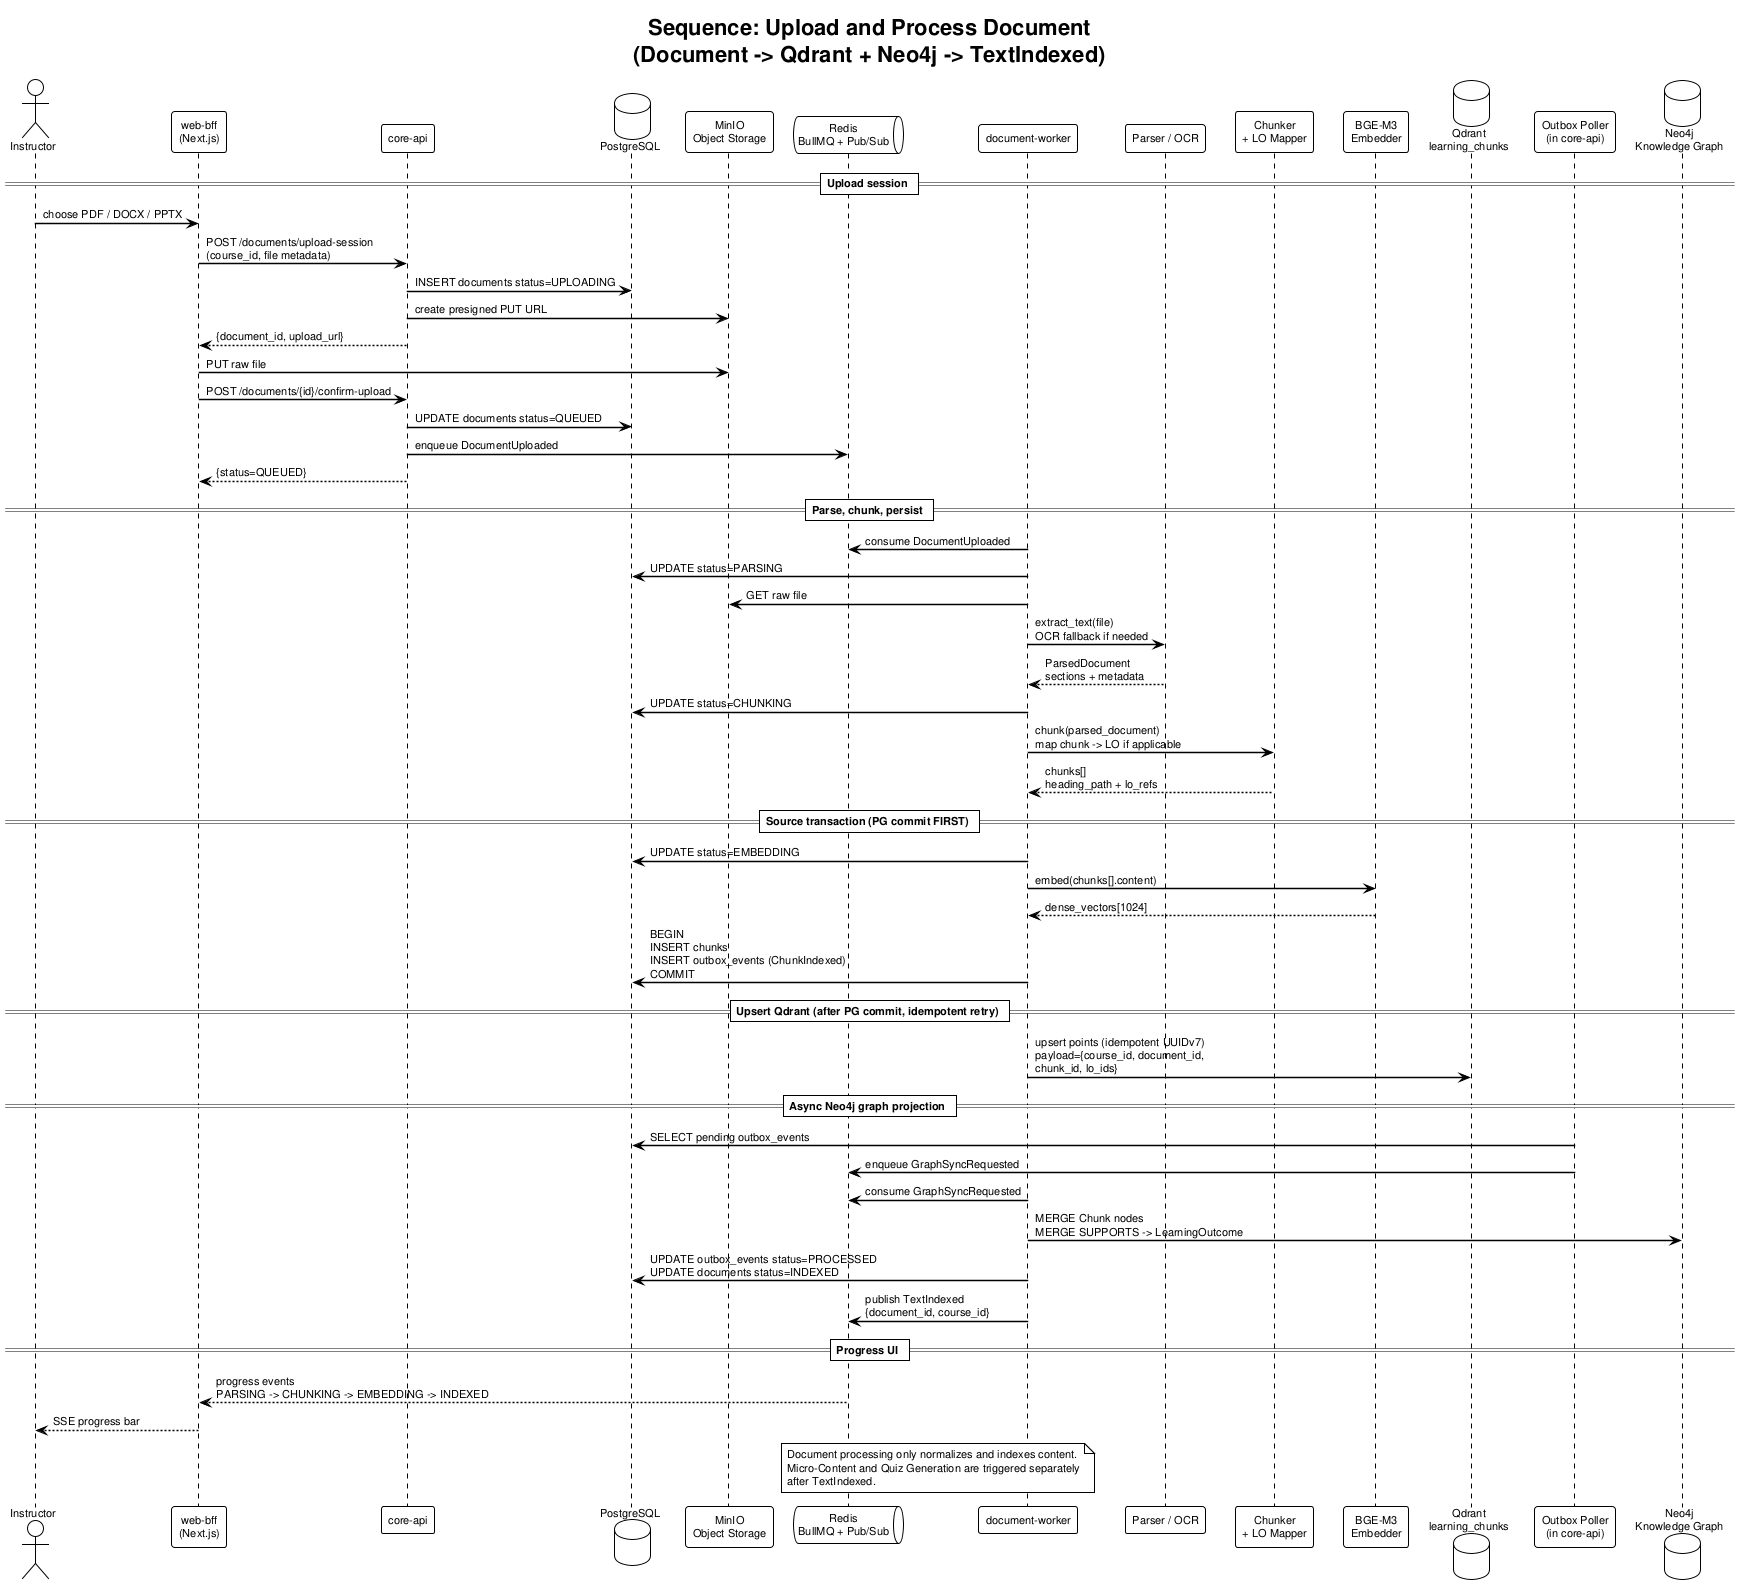
\includegraphics[width=0.95\textwidth]{diagrams/seq_document_processing.png}
    \caption{Sequence diagram for document upload and processing.}
    \label{fig:seq-document-processing}
\end{figure}

\begin{enumerate}
    \item Instructor selects PDF/DOCX/PPTX on \texttt{web-bff}.
    \item \texttt{web-bff} $\to$ \texttt{core-api}:
          \texttt{POST /documents/upload-session}.
    \item \texttt{core-api}: creates document record
          (status=UPLOADING), issues MinIO presigned URL, returns
          \texttt{document\_id}.
    \item Browser uploads directly to MinIO through presigned URL.
    \item \texttt{web-bff} $\to$ \texttt{core-api}:
          \texttt{POST /documents/\{id\}/confirm-upload}.
    \item \texttt{core-api}: update status=QUEUED, publish
          \texttt{DocumentUploaded} through BullMQ.
    \item \texttt{document-worker} (parsing) consumes event: download
          from MinIO, parse, chunk.
    \item \texttt{document-worker} (indexing): embed BGE-M3, then
          commit \texttt{chunks} and \texttt{outbox\_events}
          (\texttt{ChunkIndexed}) in one PostgreSQL transaction FIRST,
          and only after the commit upsert vectors to Qdrant (idempotent
          by UUIDv7) so no orphan vector can exist.
    \item Outbox Poller in \texttt{core-api} reads pending events and
          enqueues \texttt{GraphSyncRequested} on BullMQ.
    \item \texttt{document-worker} consumes the graph-sync job: Cypher
          \texttt{MERGE Chunk} and \texttt{SUPPORTS} relationships into
          Neo4j, then publishes \texttt{TextIndexed}.
    \item \texttt{web-bff} streams progress to browser through SSE.
\end{enumerate}

\section{Document Deletion Pipeline (Delete Saga)}
\label{appendix:delete-saga}

Requirement US-IN-11 specifies that deleting a document must remove all
derived artifacts (chunks, cards, quizzes, vector embeddings, graph
nodes, raw file) and that repeated deletion is idempotent. Because the
artifacts span five stores (PostgreSQL, Qdrant, Neo4j, MinIO, and
optionally Redis cache), this is implemented as a \emph{saga} driven by
the Outbox pattern, not by SQL \texttt{ON DELETE CASCADE} (which would
not propagate to non-relational stores).

\textbf{Step 1 - Soft delete in the source of truth.} \texttt{core-api}
handles \texttt{DELETE /documents/\{id\}} by running a single
transaction that:
\begin{itemize}
    \item sets \texttt{documents.deleted\_at = now()};
    \item soft-deletes \texttt{chunks} where
          \texttt{document\_id = :id};
    \item soft-deletes \texttt{lesson\_cards} and \texttt{quiz\_items}
          whose \texttt{source\_chunk\_ids[]} overlaps any deleted
          chunk (computed via a join against the deleted chunks set);
    \item inserts one \texttt{outbox\_events} row with
          \texttt{event\_type = DocumentDeleted} and payload
          \texttt{\{document\_id, chunk\_ids[], card\_ids[],
          quiz\_ids[]\}}.
\end{itemize}
Foreign keys remain \texttt{ON DELETE RESTRICT}; rows are never hard
deleted at this stage so the saga can replay safely.

\textbf{Step 2 - Outbox Poller dispatch.} The Outbox Poller in
\texttt{core-api} picks up \texttt{DocumentDeleted} and enqueues a
\texttt{cleanup-saga-job} on the \texttt{outbox-relay-q} queue.

\textbf{Step 3 - Cleanup worker (idempotent steps).}
\texttt{document-worker} consumes the job and runs the following steps
in order; each step is idempotent so the job can be retried at any
point:
\begin{enumerate}
    \item \texttt{Qdrant.delete(filter=\{document\_id\})} -- removes
          every vector whose payload references the deleted document.
    \item \texttt{Neo4j MATCH (c:Chunk \{document\_id\}) DETACH DELETE
          c} -- removes Chunk nodes and any \texttt{[:SUPPORTS]} edges.
    \item \texttt{MinIO.removeObject(file\_path)} -- removes the raw
          file; \texttt{NoSuchKey} errors are ignored.
    \item \texttt{Redis.DEL course:\{course\_id\}:cache:*} (best
          effort) -- invalidates any cached retrieval results.
    \item PostgreSQL update: set \texttt{outbox\_events.status =
          PROCESSED} and stamp \texttt{processed\_at}.
\end{enumerate}

\textbf{Step 4 - Optional hard delete.} After 30 days, a scheduled job
hard-deletes rows whose \texttt{deleted\_at} is older than the
retention window. Until then the soft-deleted rows preserve audit
trail and allow undo.

\textbf{Idempotency.} A re-issued \texttt{DELETE /documents/\{id\}}
returns 204 even if the document is already soft-deleted; the saga
simply finds no new outbox event to enqueue. If the cleanup worker
crashes mid-saga, retrying the job is safe because every step uses
filter-based deletion or unconditional removal.

\section{Video Upload and Processing}
\label{appendix:seq-video}

\begin{figure}[H]
    \centering
    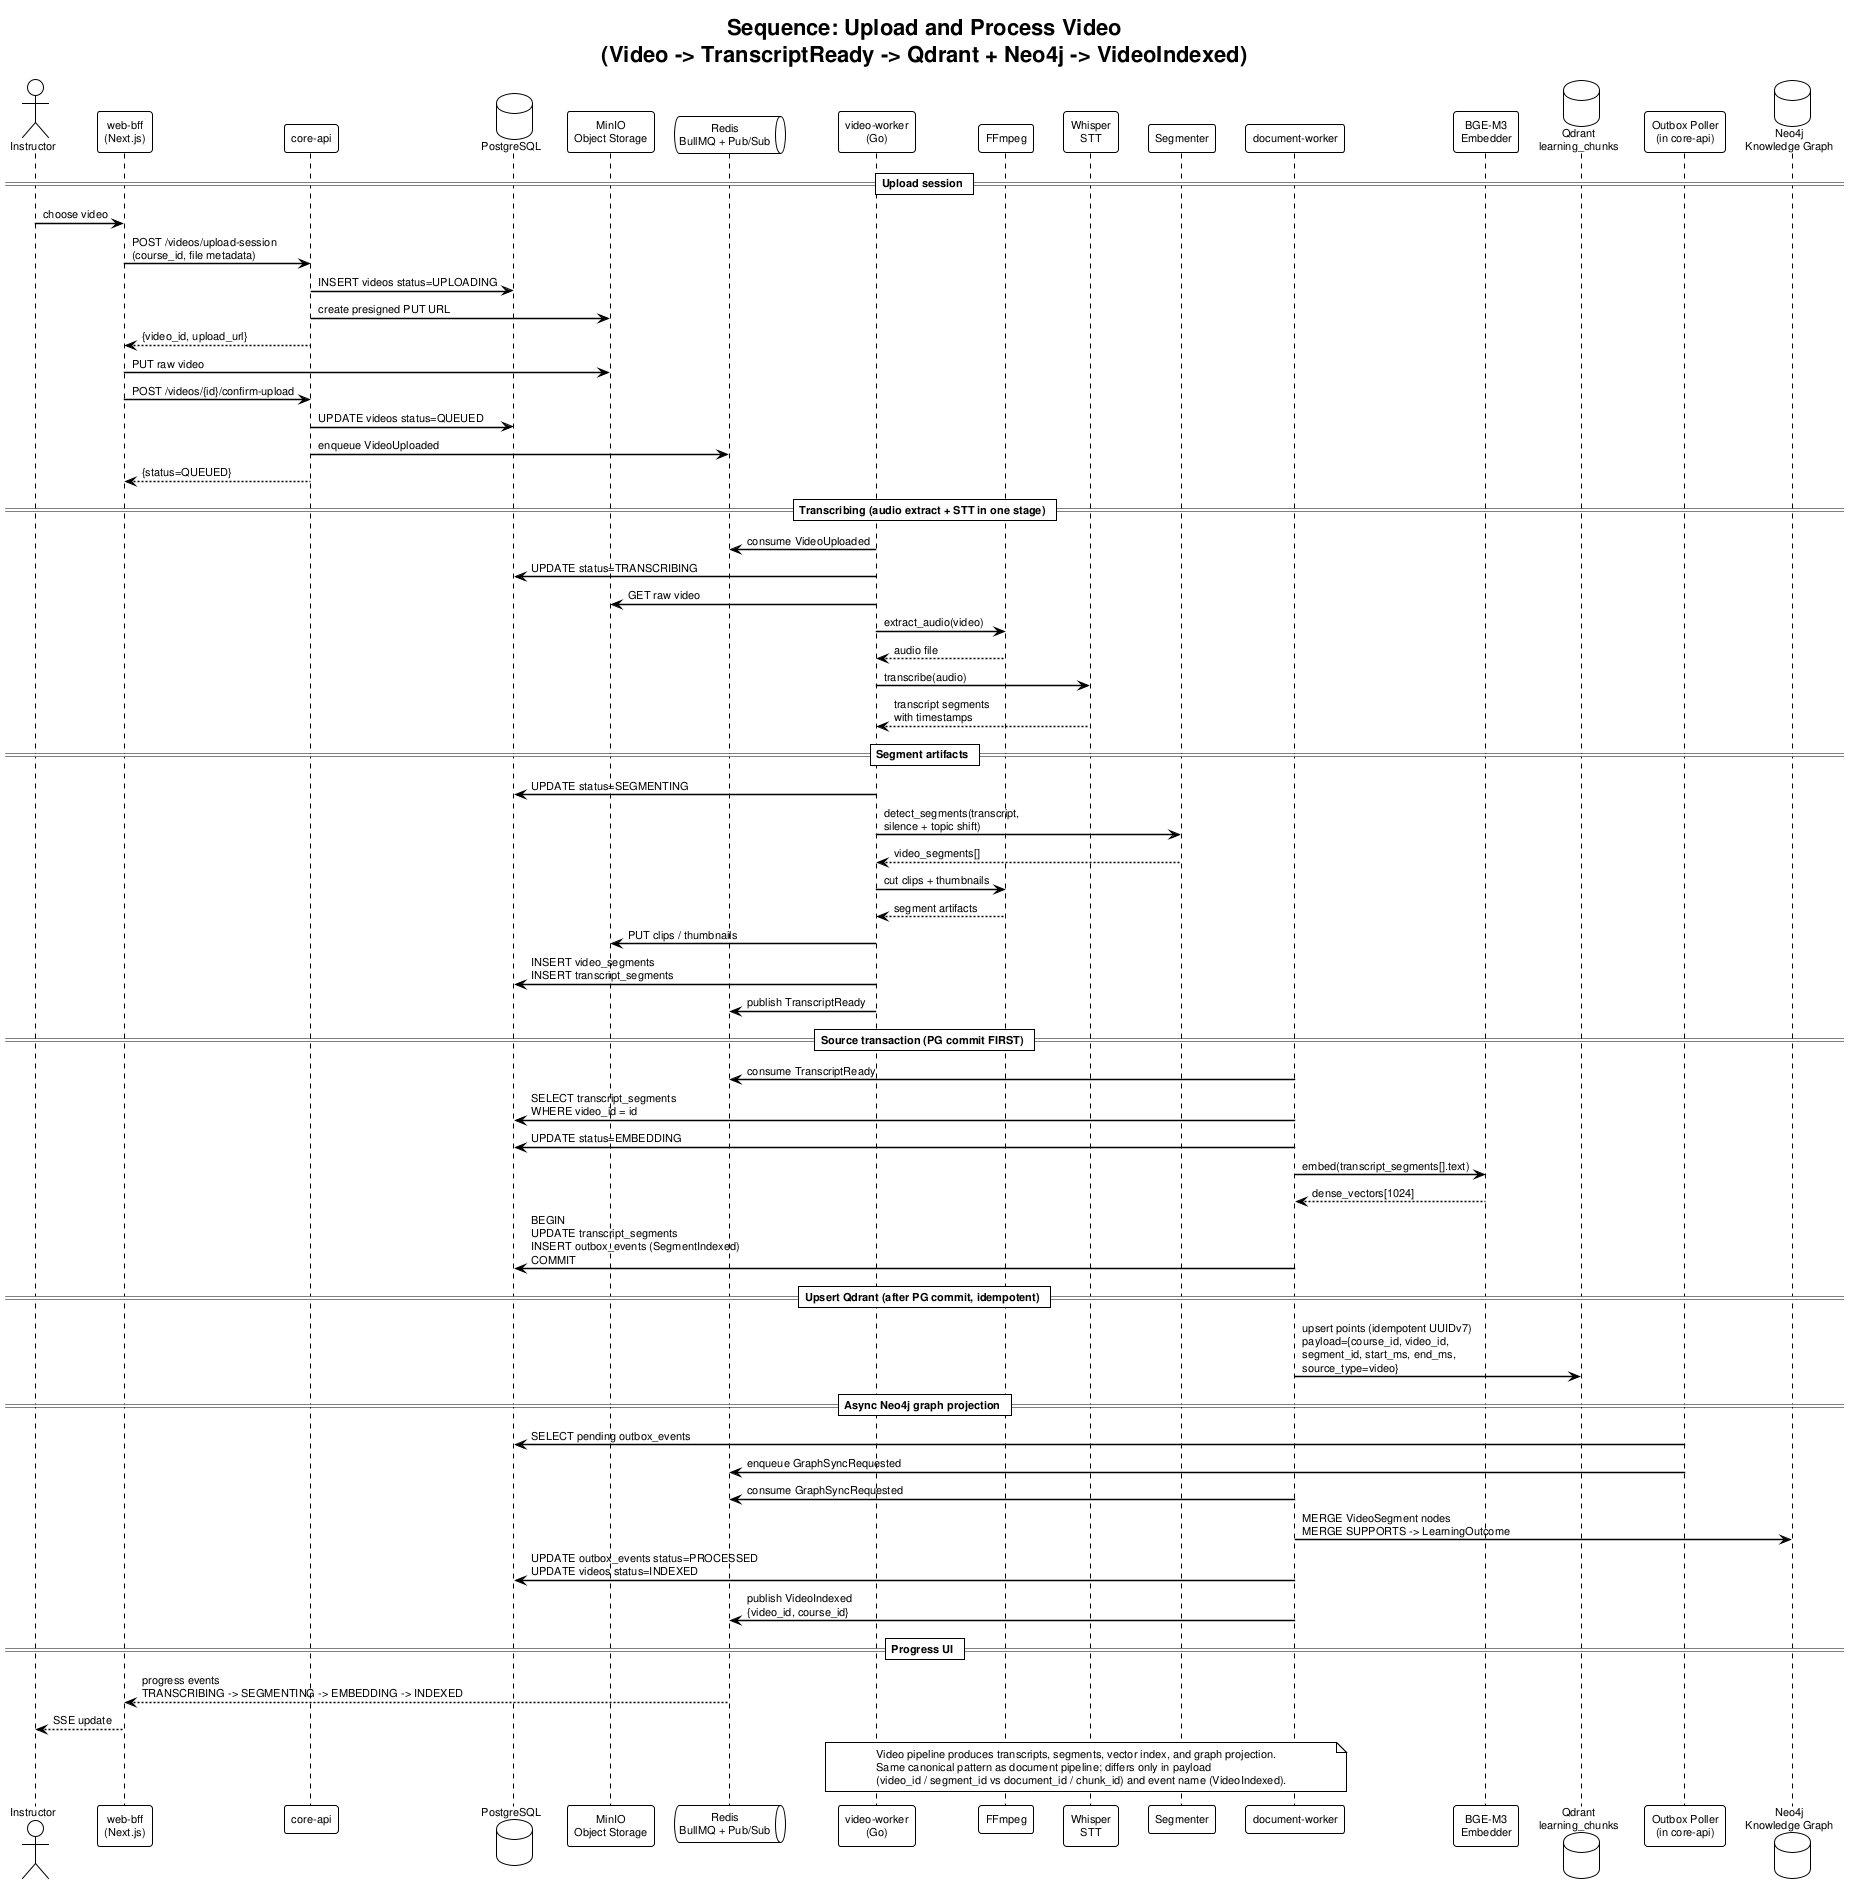
\includegraphics[width=0.95\textwidth]{diagrams/seq_video_processing.png}
    \caption{Sequence diagram for video upload and processing.}
    \label{fig:seq-video-processing}
\end{figure}

\begin{enumerate}
    \item Instructor selects a video on \texttt{web-bff}.
    \item \texttt{web-bff} $\to$ \texttt{core-api}:
          \texttt{POST /videos/upload-session}.
    \item \texttt{core-api}: creates video record, issues presigned URL,
          returns \texttt{video\_id}.
    \item Browser uploads to MinIO.
    \item \texttt{web-bff} $\to$ \texttt{core-api}: confirm upload.
    \item \texttt{core-api}: status=QUEUED, publish
          \texttt{VideoUploaded}.
    \item \texttt{video-worker} (Go) consumes: download, FFmpeg extract
          audio, Whisper transcribe, segment, cut clips, upload artifacts.
    \item Save \texttt{video\_segments}, \texttt{transcript\_segments};
          publish \texttt{TranscriptReady}.
    \item \texttt{document-worker} (indexing) consumes
          \texttt{TranscriptReady}: embed transcript, then commit
          \texttt{transcript\_segments} status and
          \texttt{outbox\_events} (\texttt{SegmentIndexed}) to
          PostgreSQL in one transaction FIRST, and only after the commit
          upsert vectors to Qdrant (idempotent by UUIDv7) so no orphan
          vector can exist.
    \item Outbox Poller in \texttt{core-api} dispatches
          \texttt{GraphSyncRequested}; \texttt{document-worker} projects
          \texttt{VideoSegment} nodes and \texttt{SUPPORTS} relations
          into Neo4j, then publishes \texttt{VideoIndexed}.
\end{enumerate}

\section{AI Tutor Chatbot}
\label{appendix:seq-chatbot}

\begin{figure}[H]
    \centering
    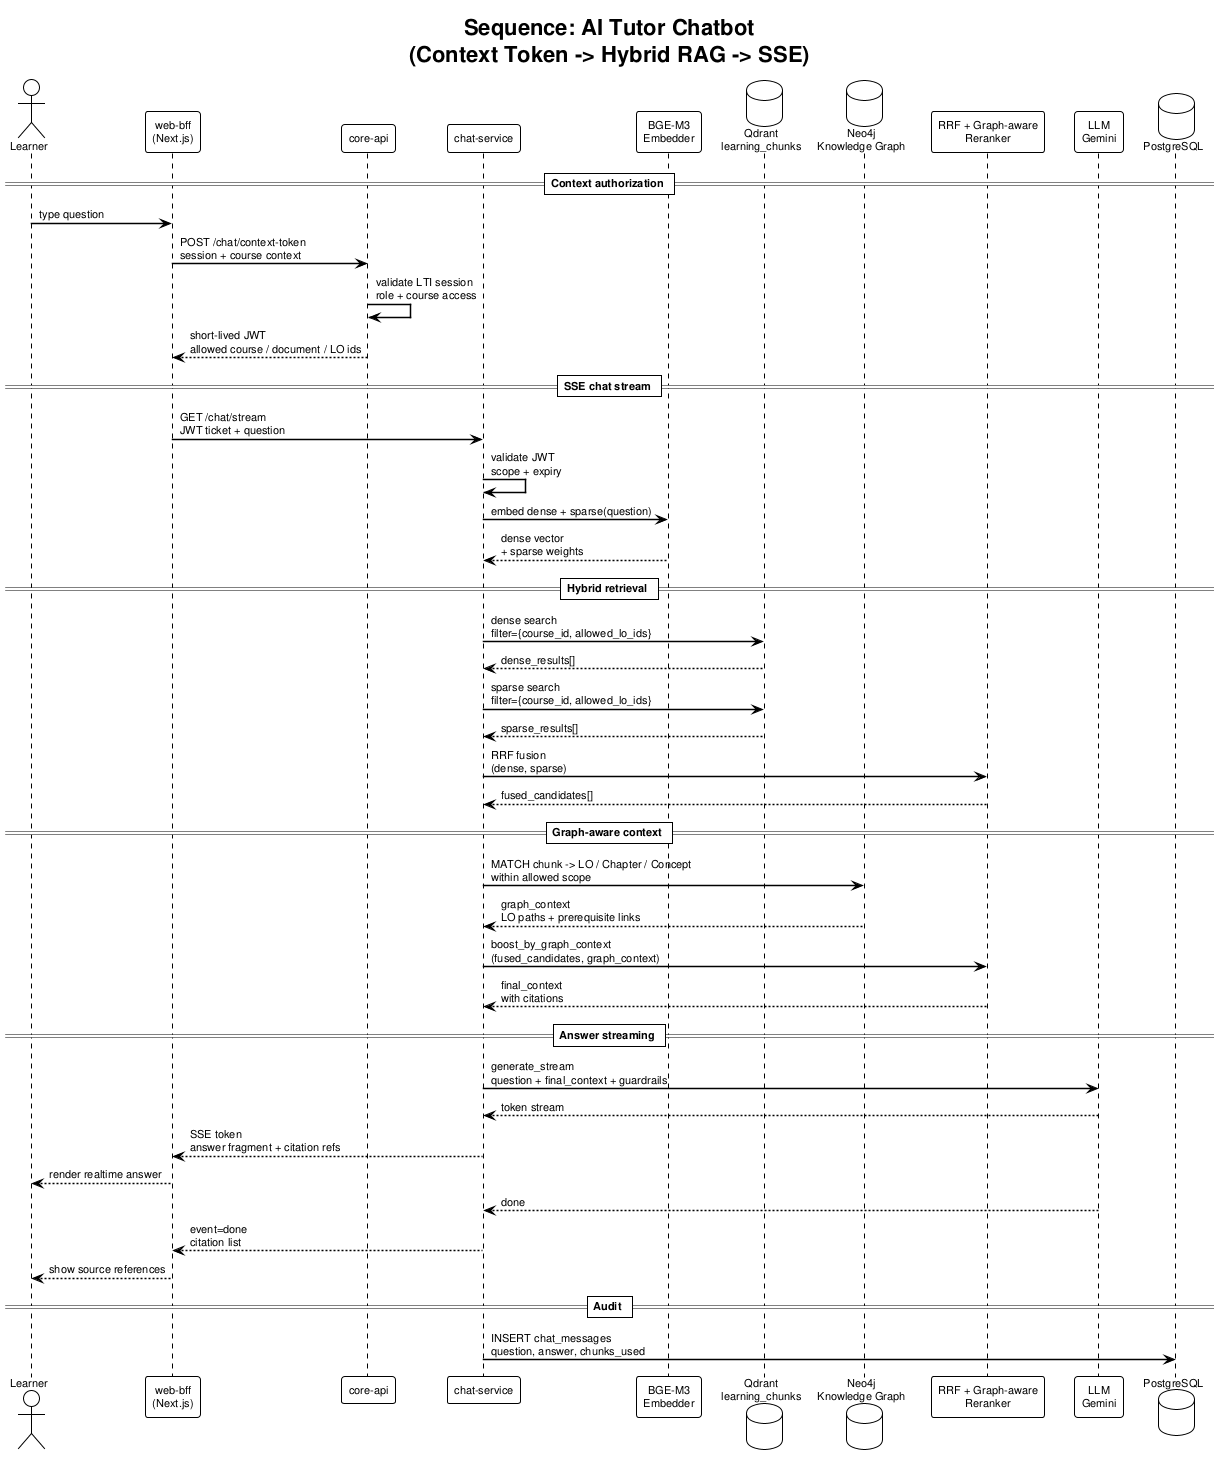
\includegraphics[width=0.95\textwidth]{diagrams/seq_ai_tutor_chatbot.png}
    \caption{Sequence diagram for the AI Tutor Chatbot.}
    \label{fig:seq-ai-tutor-chatbot}
\end{figure}

\begin{enumerate}
    \item Learner sends a question on \texttt{web-bff}.
    \item \texttt{web-bff} $\to$ \texttt{core-api}:
          \texttt{POST /chat/context-token} with session info.
    \item \texttt{core-api}: validate session, generate short-lived JWT
          containing \texttt{user\_id}, \texttt{course\_id},
          \texttt{allowed\_document\_ids}, \texttt{allowed\_lo\_ids}.
    \item \texttt{web-bff} opens SSE to \texttt{chat-service}
          \texttt{/chat/stream} with token + question.
    \item \texttt{chat-service}: validate token, embed question, search
          Qdrant top-K with course/LO filter.
    \item If the question is LO-related: query Neo4j for chunks
          \texttt{SUPPORTS} LO and rerank.
    \item Build prompt with context + citation, call LLM streaming.
    \item For every token received, \texttt{chat-service} pushes through
          SSE; \texttt{web-bff} forwards to browser.
    \item On completion: send \texttt{event: done} with citation list and
          save chat message in PostgreSQL.
\end{enumerate}

\section{Quiz Generation}
\label{appendix:seq-quiz}

\begin{figure}[H]
    \centering
    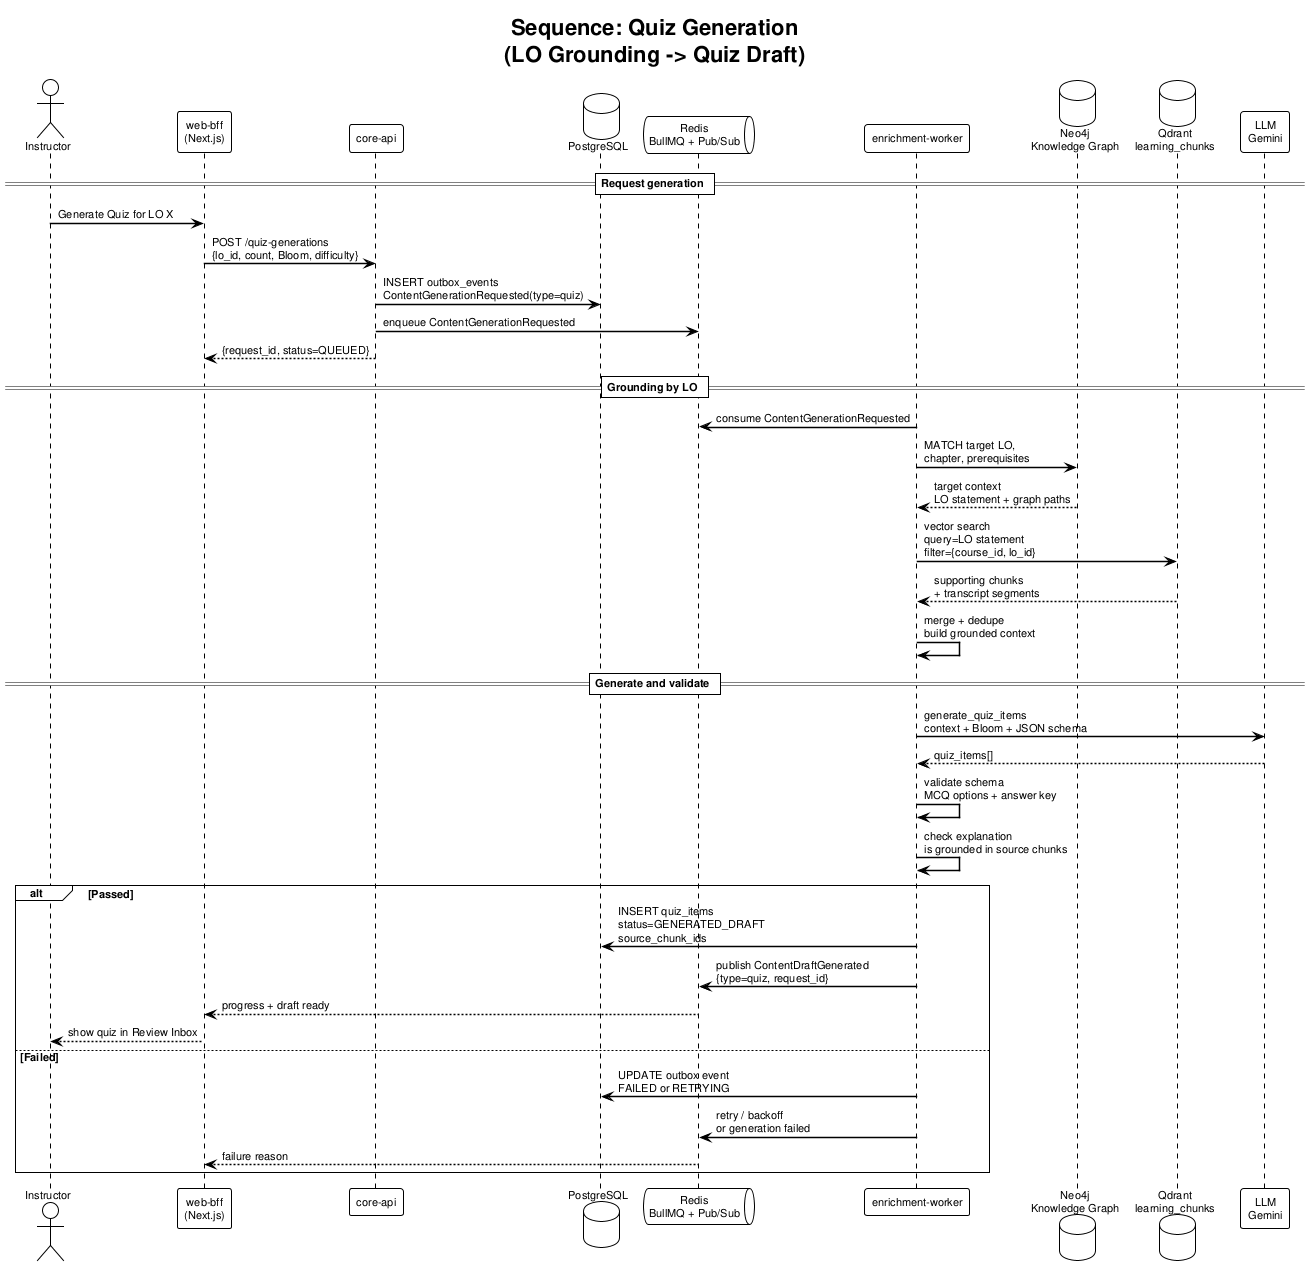
\includegraphics[width=0.95\textwidth]{diagrams/seq_quiz_generation.png}
    \caption{Sequence diagram for quiz generation.}
    \label{fig:seq-quiz-generation}
\end{figure}

The full step-by-step description is given in
Section~\ref{subsec:quiz-pipeline} of Chapter~\ref{chap:phan-tich-thiet-ke};
this appendix provides the corresponding sequence diagram for
defense-day reference.

\section{Curriculum Ingestion}
\label{appendix:seq-curriculum}

\begin{figure}[H]
    \centering
    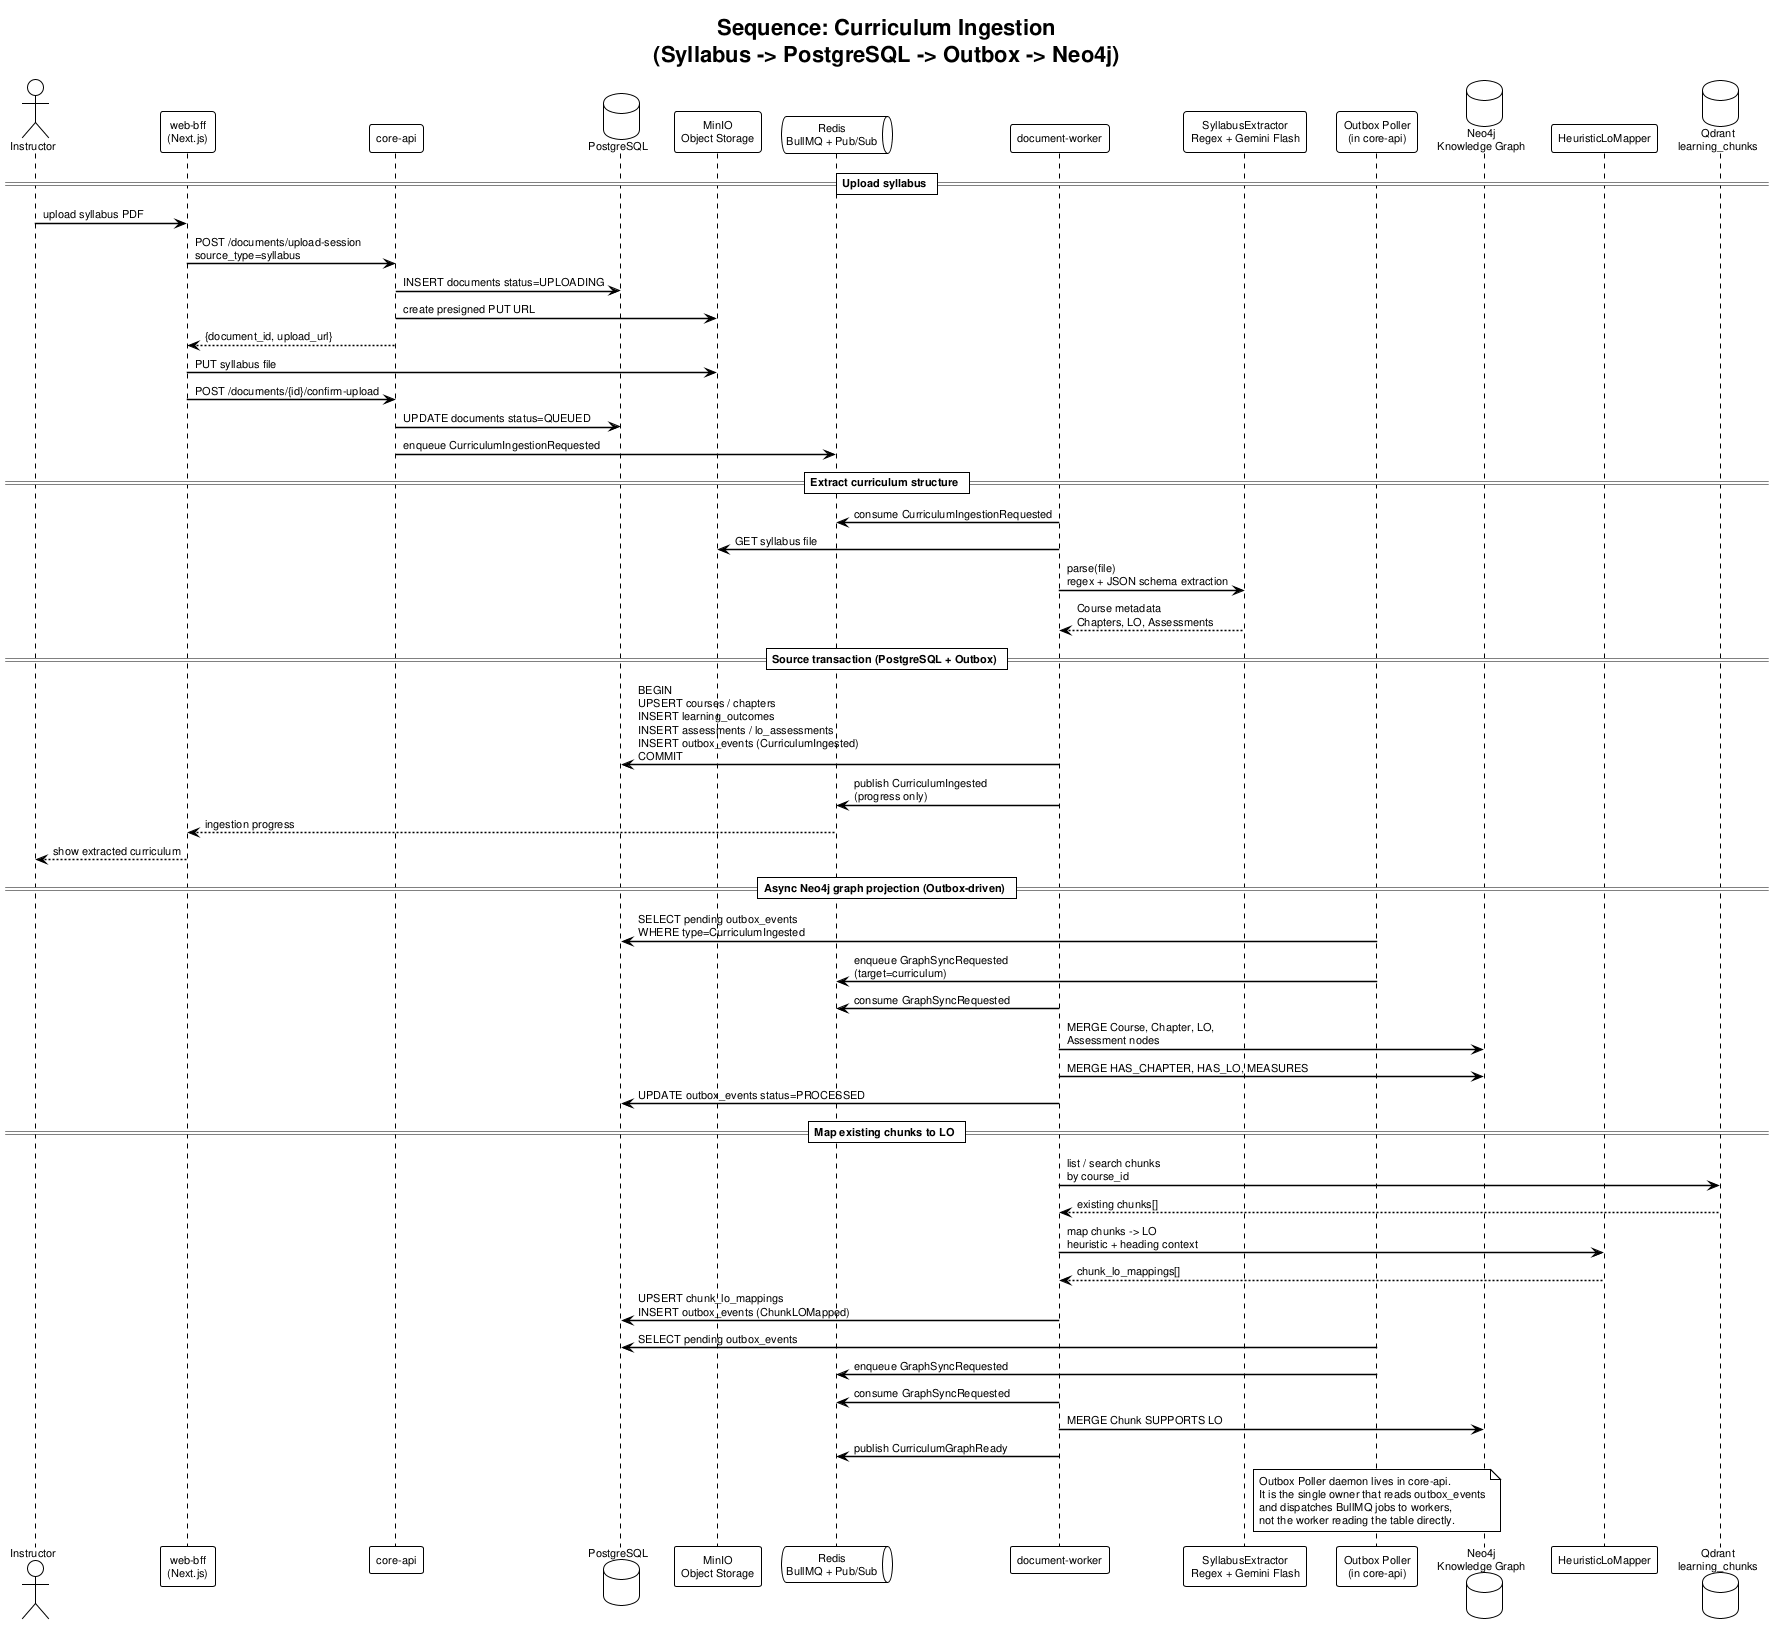
\includegraphics[width=0.95\textwidth]{diagrams/seq_curriculum_ingestion.png}
    \caption{Sequence diagram for ingesting the course syllabus.}
    \label{fig:seq-ingest-curriculum-lvtn}
\end{figure}

\begin{enumerate}
    \item Instructor uploads the syllabus PDF through \texttt{web-bff}.
    \item Upload session $\to$ MinIO $\to$ confirm, like the document flow.
    \item \texttt{core-api}: publish
          \texttt{CurriculumIngestionRequested} with
          \texttt{document\_id}, \texttt{course\_id}.
    \item \texttt{document-worker} (curriculum): download the syllabus,
          call \texttt{SyllabusExtractor} hybrid parse (Regex + Gemini
          Flash JSON schema).
    \item Extract Course metadata, Chapter list, Learning Outcome (LO),
          Assessment.
    \item Insert PostgreSQL in one transaction: \texttt{courses},
          \texttt{chapters}, \texttt{learning\_outcomes},
          \texttt{assessments}, \texttt{lo\_assessments}.
    \item In the same transaction: insert \texttt{outbox\_events} with
          \texttt{CurriculumIngested} payload.
    \item Outbox Poller daemon in \texttt{core-api} reads the event and
          pushes a job to \texttt{document-worker} to project into Neo4j:
          create Course, Chapter, LO, Assessment nodes and relationships
          \texttt{HAS\_CHAPTER}, \texttt{HAS\_LO}, \texttt{MEASURES}.
    \item After LO graph exists: \texttt{HeuristicLoMapper} runs on all
          existing chunks of the course, creating
          \texttt{chunk\_lo\_mappings} and \texttt{SUPPORTS}
          relationships.
\end{enumerate}
